\documentclass[11pt]{article}
\usepackage[textwidth=18.0cm, textheight=23.0cm, top=2.0cm]{geometry}
\usepackage{pst-all}
\usepackage{amssymb}
\usepackage{tikz}
\usepackage{underscore}\begin{document}
\pagestyle{empty}


ClassName: \underline{\textbf{Class_07.2bp-10}}
\par
BinSize: \underline{\textbf{100 × 100}}
\par
ReduceSize: \underline{\textbf{100 × 100}}
\par
TypeNum: \underline{\textbf{38}}
\par
Num: \underline{\textbf{40}}
\par
OutS: \underline{\textbf{100000}}
\par
InS: \underline{\textbf{83538}}
\par
Rate: \underline{\textbf{0.835}}
\par
UB: \underline{\textbf{10}}
\par
LB0: \underline{\textbf{10}}
\par
LB: \underline{\textbf{10}}
\par
LBWithCut: \underline{\textbf{10}}
\par
NodeCut: \underline{\textbf{0}}
\par
ExtendedNodeCnt: \underline{\textbf{1}}
\par
GenNodeCnt: \underline{\textbf{1}}
\par
PrimalNode: \underline{\textbf{0}}
\par
ColumnCount: \underline{\textbf{10}}
\par
TotalCutCount: \underline{\textbf{0}}
\par
RootCutCount: \underline{\textbf{0}}
\par
LPSolverCnt: \underline{\textbf{1}}
\par
PricingSolverCnt: \underline{\textbf{0}}
\par
BranchAndBoundNum: \underline{\textbf{1}}
\par
isOpt: \underline{\textbf{true}}
\par
TimeOnPrimal: \underline{\textbf{0.000 s}}
\par
TimeOnPricing: \underline{\textbf{0.000 s}}
\par
TimeOnRmp: \underline{\textbf{0.079 s}}
\par
TotalTime: \underline{\textbf{0.141 s}}
\par
\newpage


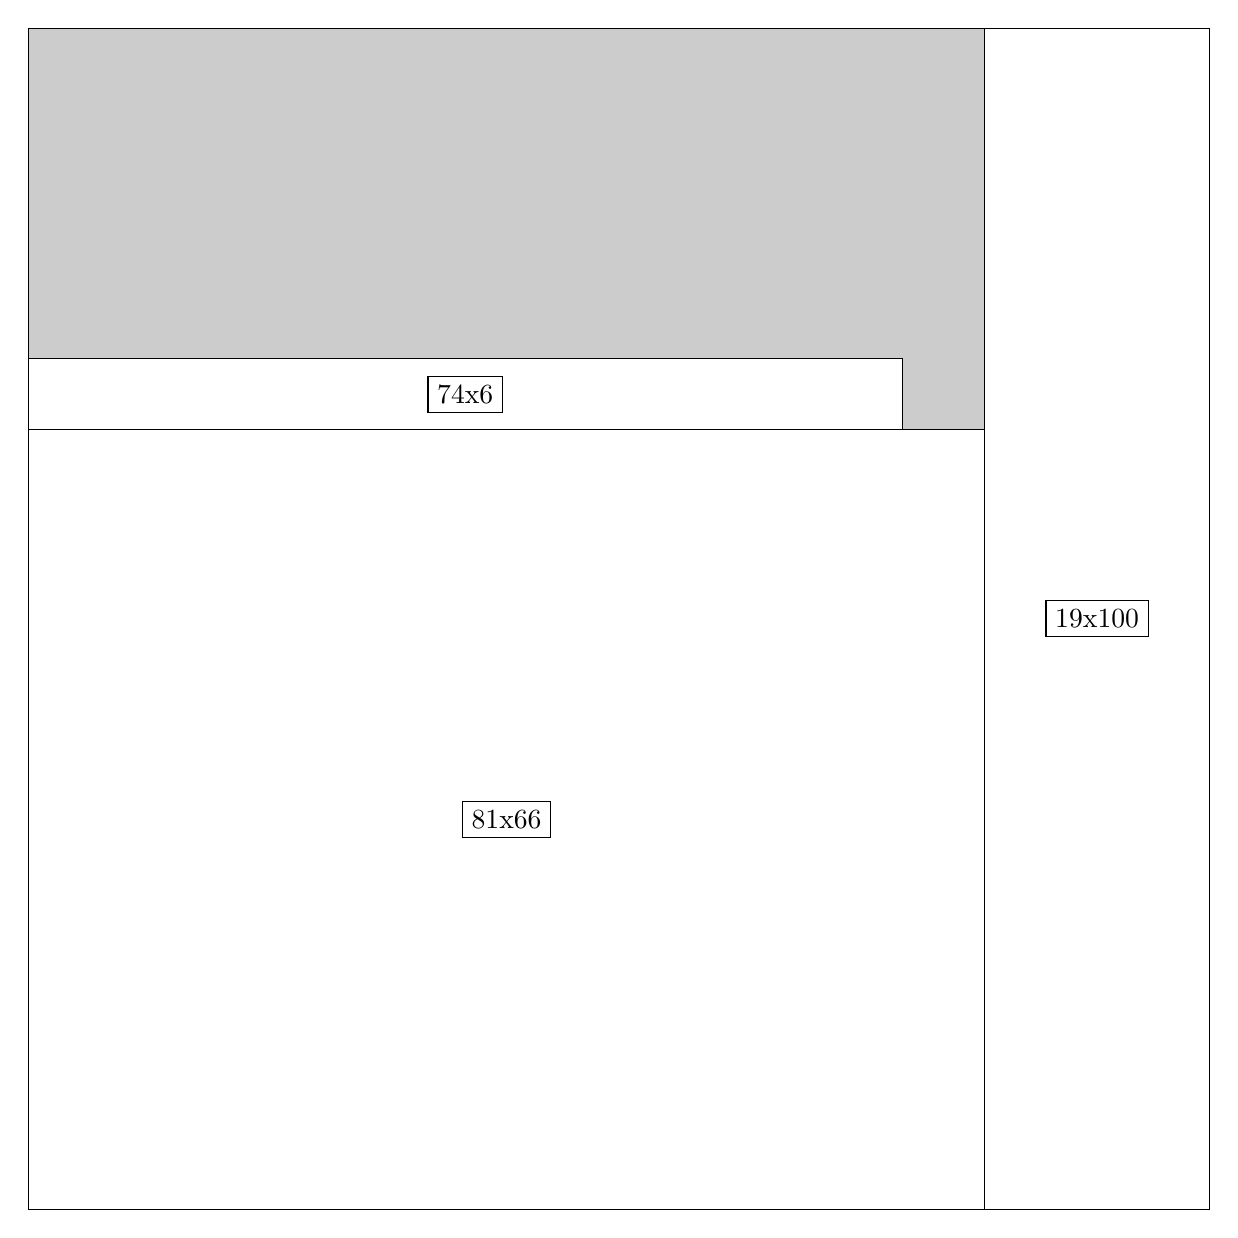
\begin{tikzpicture}[shorten >=1pt,scale=1.0,every node/.style={scale=1.0},->]
\tikzstyle{vertex}=[circle,fill=black!25,minimum size=14pt,inner sep=0pt]
\filldraw[fill=gray!40!white, draw=black] (0,0) rectangle (15.0,15.0);
\foreach \name/\x/\y/\w/\h in {81x66/0.0/0.0/12.15/9.9,19x100/12.15/0.0/2.85/15.0,74x6/0.0/9.9/11.1/0.8999999999999999}
\filldraw[fill=white!40!white, draw=black] (\x,\y) rectangle node[draw] (\name) {\name} ++(\w,\h);
\end{tikzpicture}


w =81 , h =66 , x =0 , y =0 , v =5346
\par
w =19 , h =100 , x =81 , y =0 , v =1900
\par
w =74 , h =6 , x =0 , y =66 , v =444
\par
\newpage


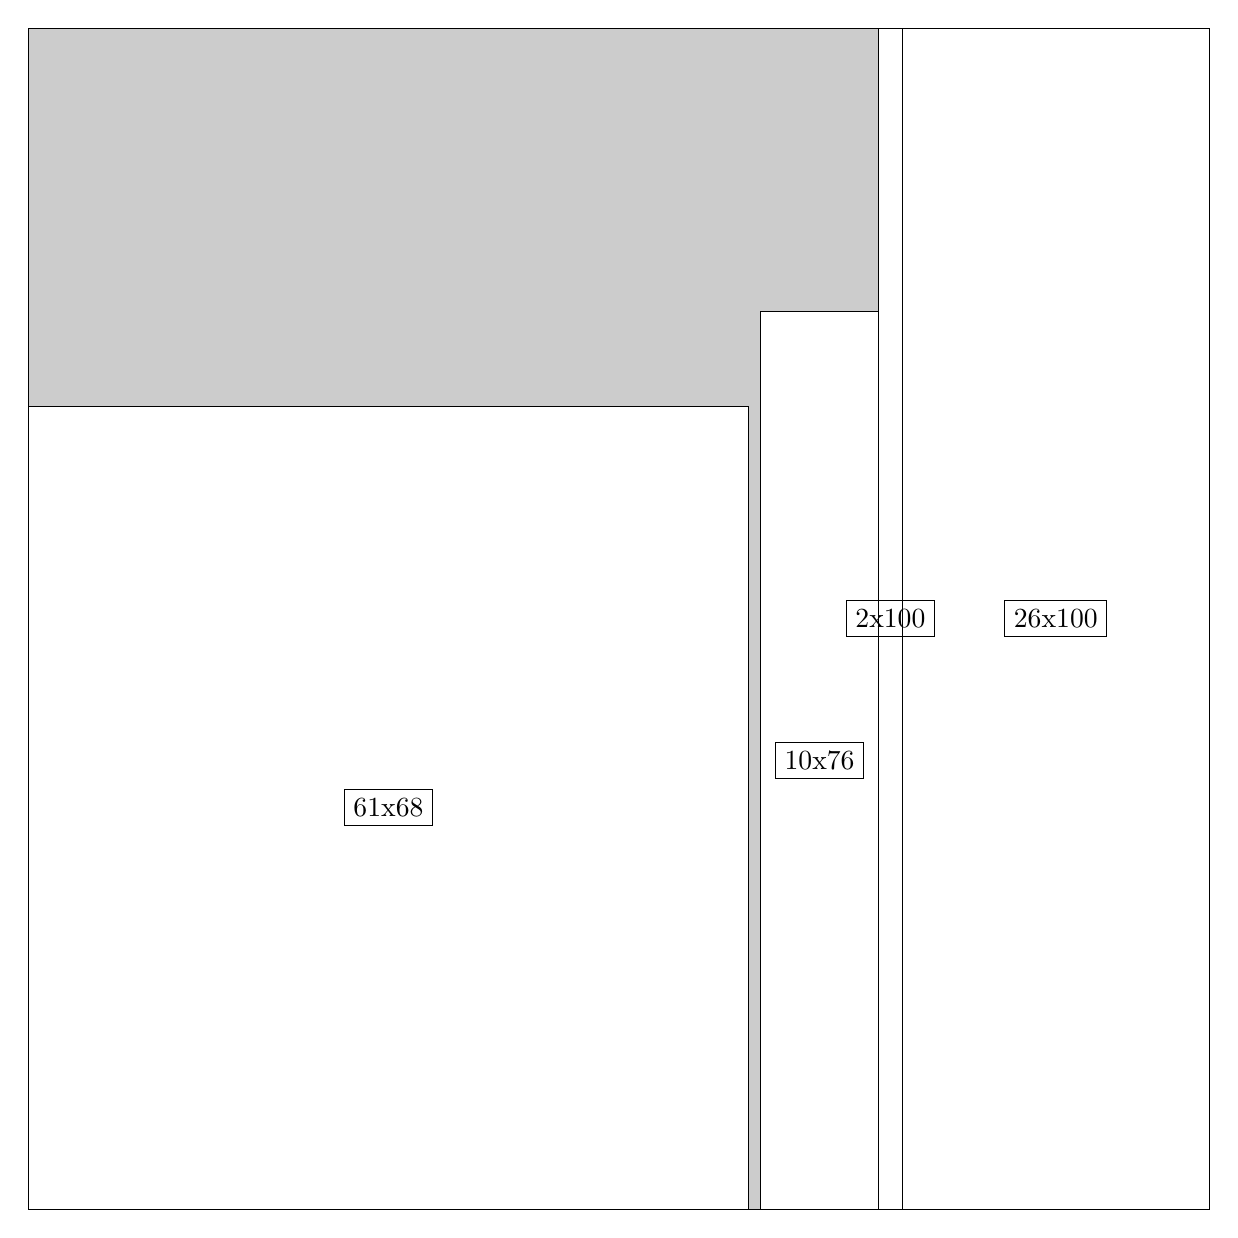
\begin{tikzpicture}[shorten >=1pt,scale=1.0,every node/.style={scale=1.0},->]
\tikzstyle{vertex}=[circle,fill=black!25,minimum size=14pt,inner sep=0pt]
\filldraw[fill=gray!40!white, draw=black] (0,0) rectangle (15.0,15.0);
\foreach \name/\x/\y/\w/\h in {61x68/0.0/0.0/9.15/10.2,26x100/11.1/0.0/3.9/15.0,10x76/9.299999999999999/0.0/1.5/11.4,2x100/10.799999999999999/0.0/0.3/15.0}
\filldraw[fill=white!40!white, draw=black] (\x,\y) rectangle node[draw] (\name) {\name} ++(\w,\h);
\end{tikzpicture}


w =61 , h =68 , x =0 , y =0 , v =4148
\par
w =26 , h =100 , x =74 , y =0 , v =2600
\par
w =10 , h =76 , x =62 , y =0 , v =760
\par
w =2 , h =100 , x =72 , y =0 , v =200
\par
\newpage


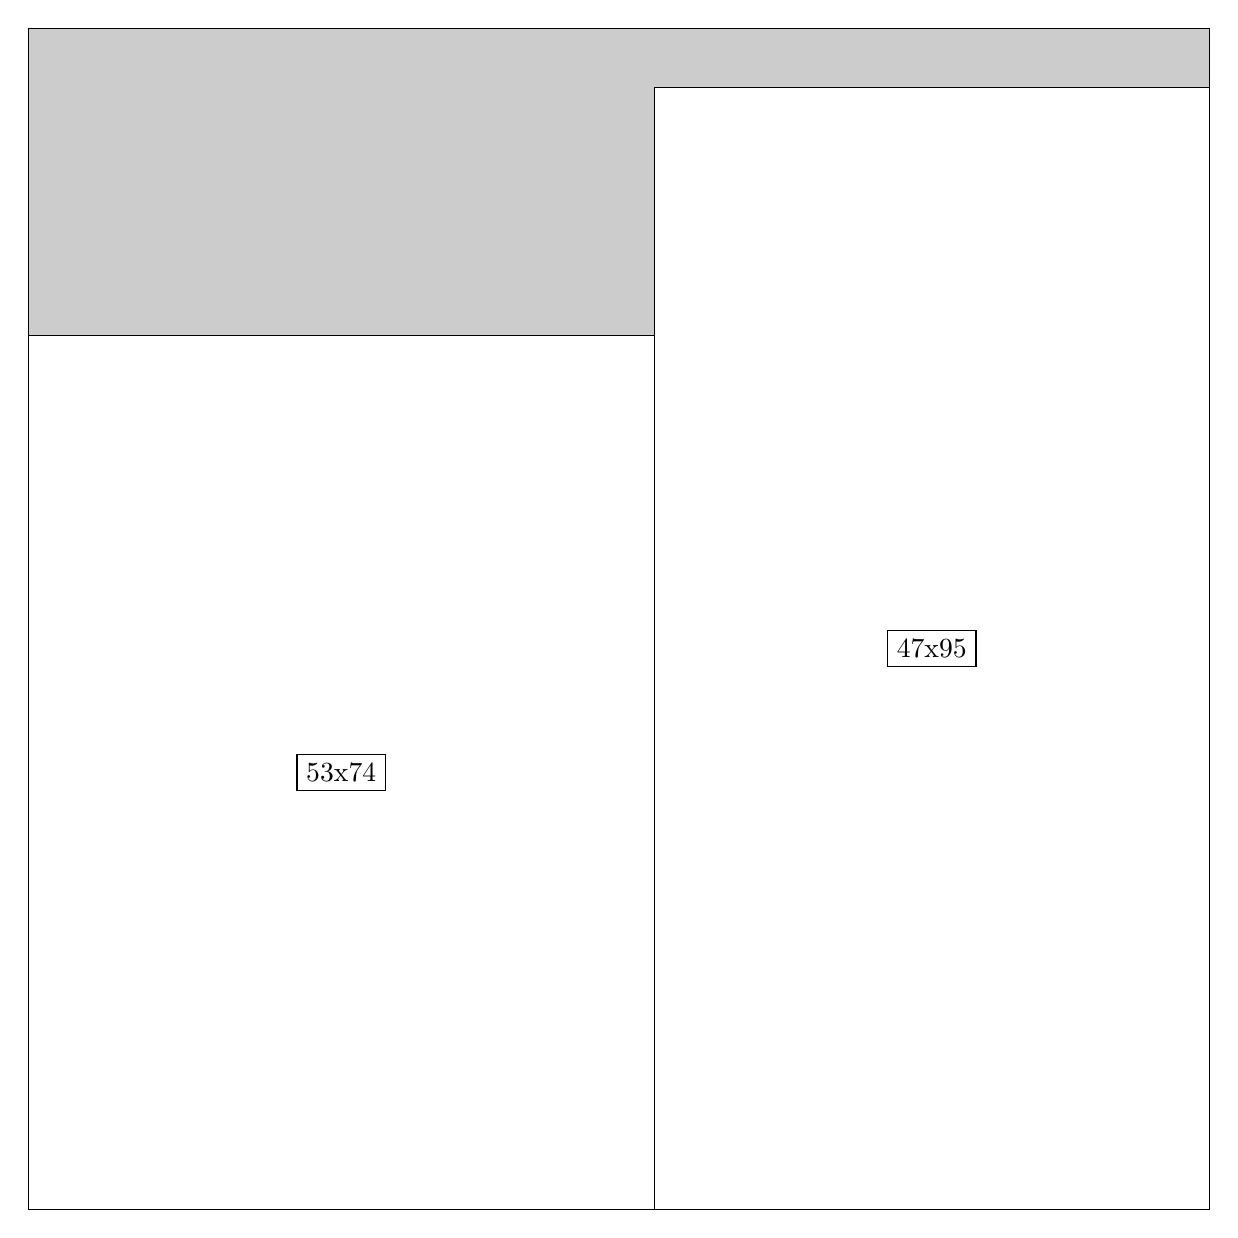
\begin{tikzpicture}[shorten >=1pt,scale=1.0,every node/.style={scale=1.0},->]
\tikzstyle{vertex}=[circle,fill=black!25,minimum size=14pt,inner sep=0pt]
\filldraw[fill=gray!40!white, draw=black] (0,0) rectangle (15.0,15.0);
\foreach \name/\x/\y/\w/\h in {47x95/7.949999999999999/0.0/7.05/14.25,53x74/0.0/0.0/7.949999999999999/11.1}
\filldraw[fill=white!40!white, draw=black] (\x,\y) rectangle node[draw] (\name) {\name} ++(\w,\h);
\end{tikzpicture}


w =47 , h =95 , x =53 , y =0 , v =4465
\par
w =53 , h =74 , x =0 , y =0 , v =3922
\par
\newpage


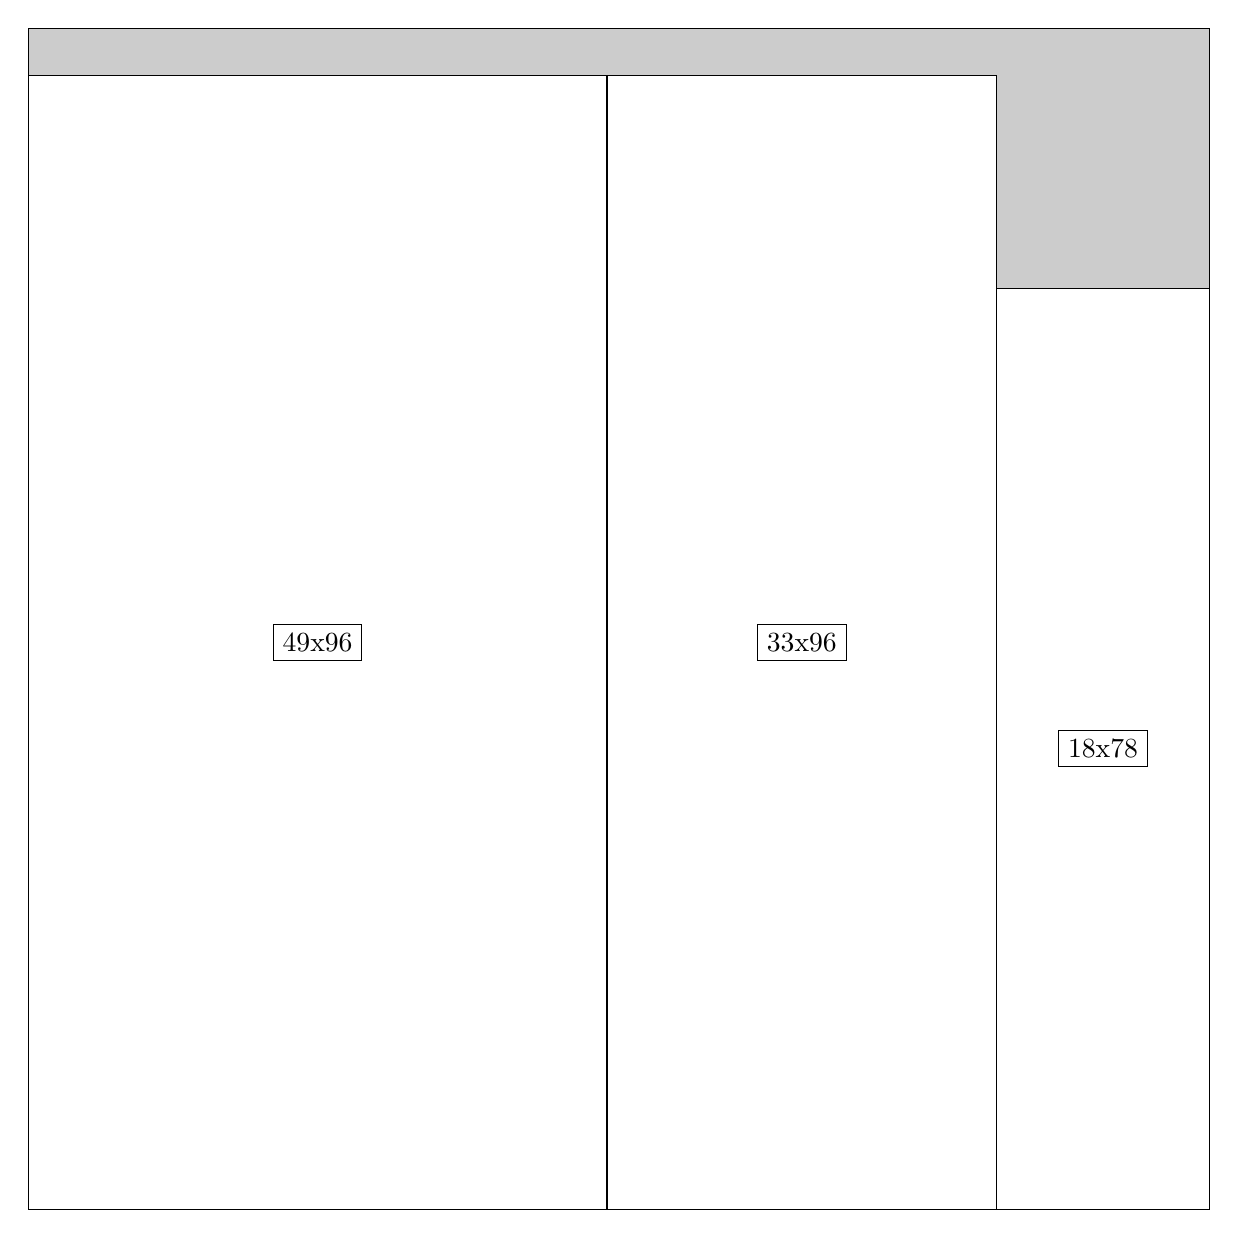
\begin{tikzpicture}[shorten >=1pt,scale=1.0,every node/.style={scale=1.0},->]
\tikzstyle{vertex}=[circle,fill=black!25,minimum size=14pt,inner sep=0pt]
\filldraw[fill=gray!40!white, draw=black] (0,0) rectangle (15.0,15.0);
\foreach \name/\x/\y/\w/\h in {49x96/0.0/0.0/7.35/14.399999999999999,33x96/7.35/0.0/4.95/14.399999999999999,18x78/12.299999999999999/0.0/2.6999999999999997/11.7}
\filldraw[fill=white!40!white, draw=black] (\x,\y) rectangle node[draw] (\name) {\name} ++(\w,\h);
\end{tikzpicture}


w =49 , h =96 , x =0 , y =0 , v =4704
\par
w =33 , h =96 , x =49 , y =0 , v =3168
\par
w =18 , h =78 , x =82 , y =0 , v =1404
\par
\newpage


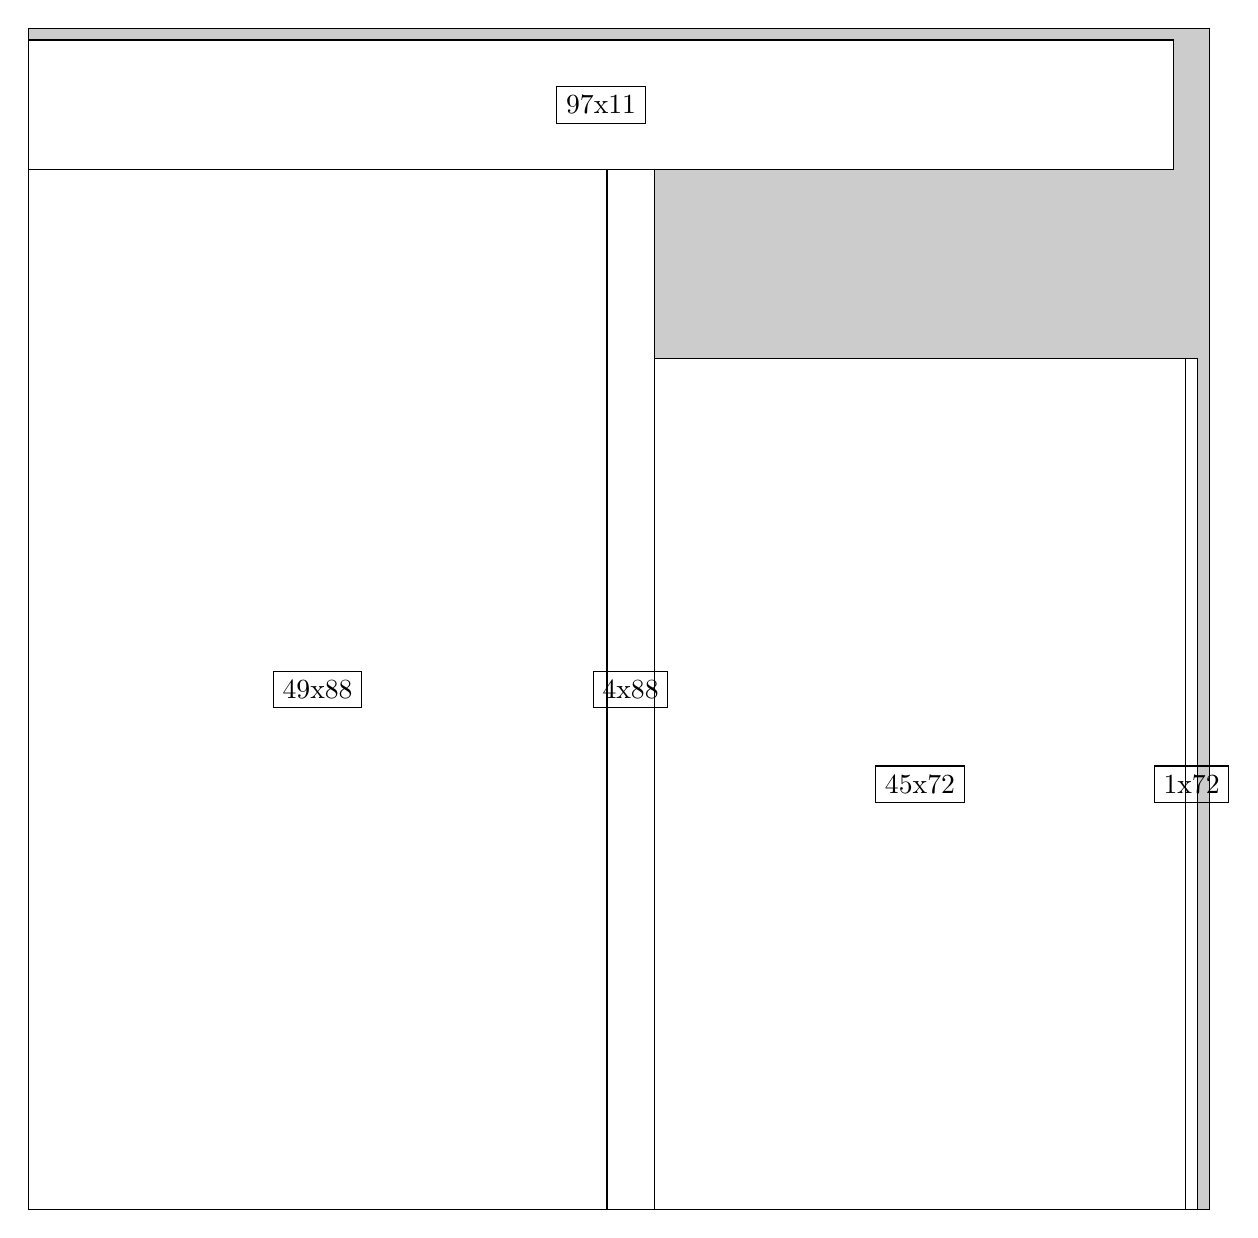
\begin{tikzpicture}[shorten >=1pt,scale=1.0,every node/.style={scale=1.0},->]
\tikzstyle{vertex}=[circle,fill=black!25,minimum size=14pt,inner sep=0pt]
\filldraw[fill=gray!40!white, draw=black] (0,0) rectangle (15.0,15.0);
\foreach \name/\x/\y/\w/\h in {49x88/0.0/0.0/7.35/13.2,45x72/7.949999999999999/0.0/6.75/10.799999999999999,97x11/0.0/13.2/14.549999999999999/1.65,4x88/7.35/0.0/0.6/13.2,1x72/14.7/0.0/0.15/10.799999999999999}
\filldraw[fill=white!40!white, draw=black] (\x,\y) rectangle node[draw] (\name) {\name} ++(\w,\h);
\end{tikzpicture}


w =49 , h =88 , x =0 , y =0 , v =4312
\par
w =45 , h =72 , x =53 , y =0 , v =3240
\par
w =97 , h =11 , x =0 , y =88 , v =1067
\par
w =4 , h =88 , x =49 , y =0 , v =352
\par
w =1 , h =72 , x =98 , y =0 , v =72
\par
\newpage


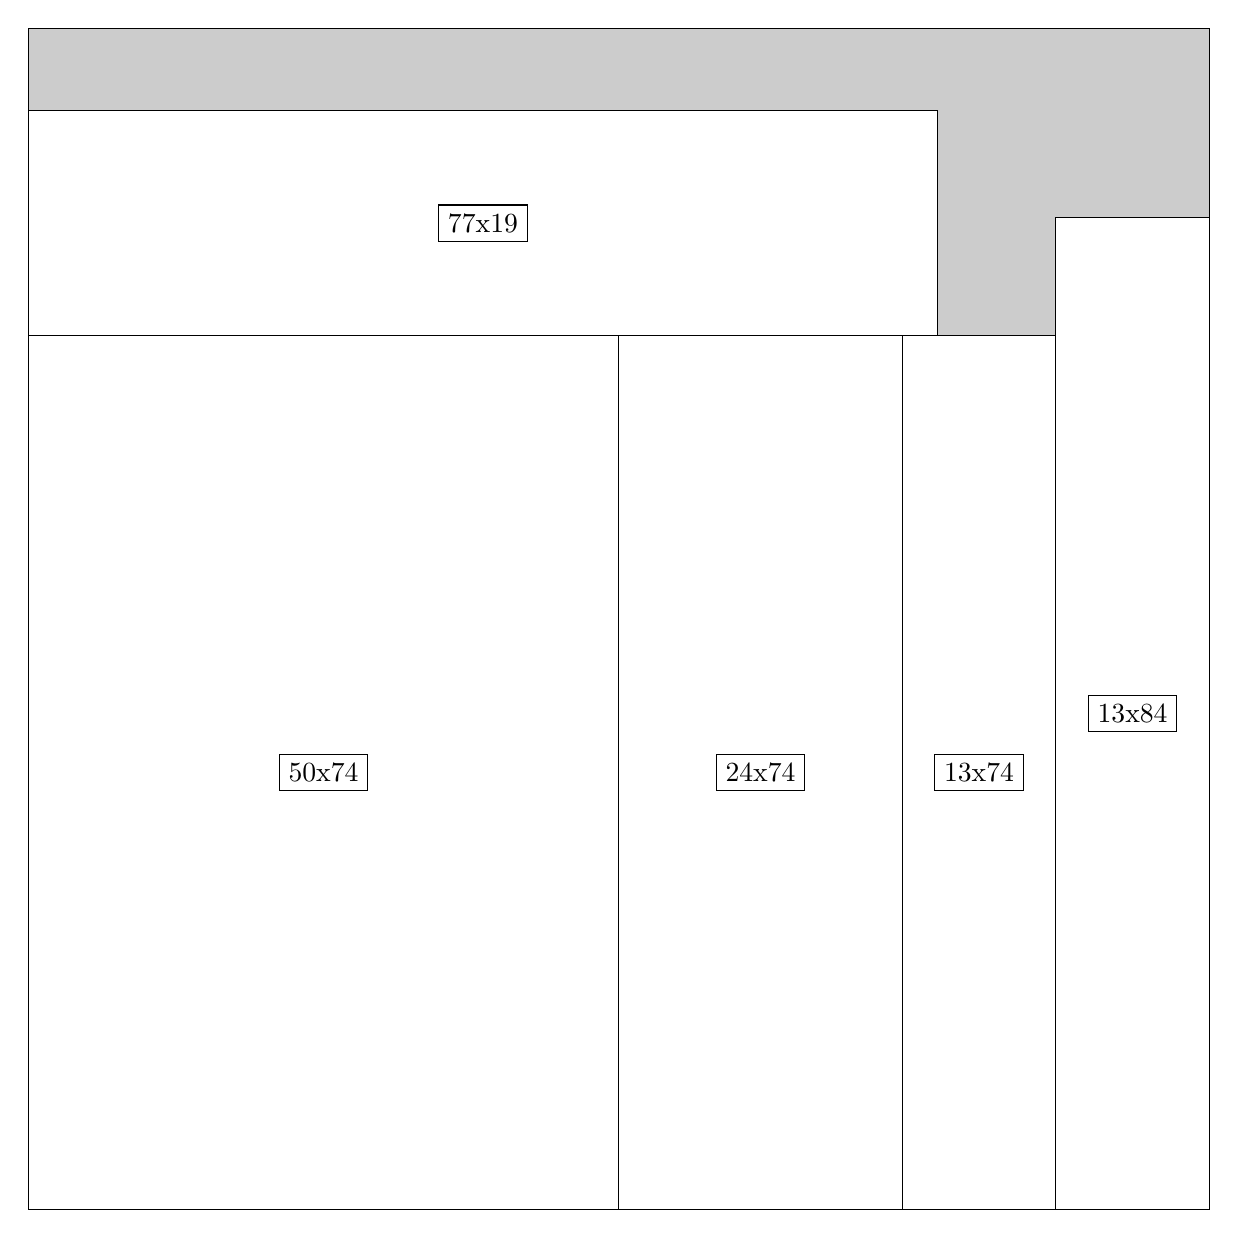
\begin{tikzpicture}[shorten >=1pt,scale=1.0,every node/.style={scale=1.0},->]
\tikzstyle{vertex}=[circle,fill=black!25,minimum size=14pt,inner sep=0pt]
\filldraw[fill=gray!40!white, draw=black] (0,0) rectangle (15.0,15.0);
\foreach \name/\x/\y/\w/\h in {50x74/0.0/0.0/7.5/11.1,24x74/7.5/0.0/3.5999999999999996/11.1,77x19/0.0/11.1/11.549999999999999/2.85,13x84/13.049999999999999/0.0/1.95/12.6,13x74/11.1/0.0/1.95/11.1}
\filldraw[fill=white!40!white, draw=black] (\x,\y) rectangle node[draw] (\name) {\name} ++(\w,\h);
\end{tikzpicture}


w =50 , h =74 , x =0 , y =0 , v =3700
\par
w =24 , h =74 , x =50 , y =0 , v =1776
\par
w =77 , h =19 , x =0 , y =74 , v =1463
\par
w =13 , h =84 , x =87 , y =0 , v =1092
\par
w =13 , h =74 , x =74 , y =0 , v =962
\par
\newpage


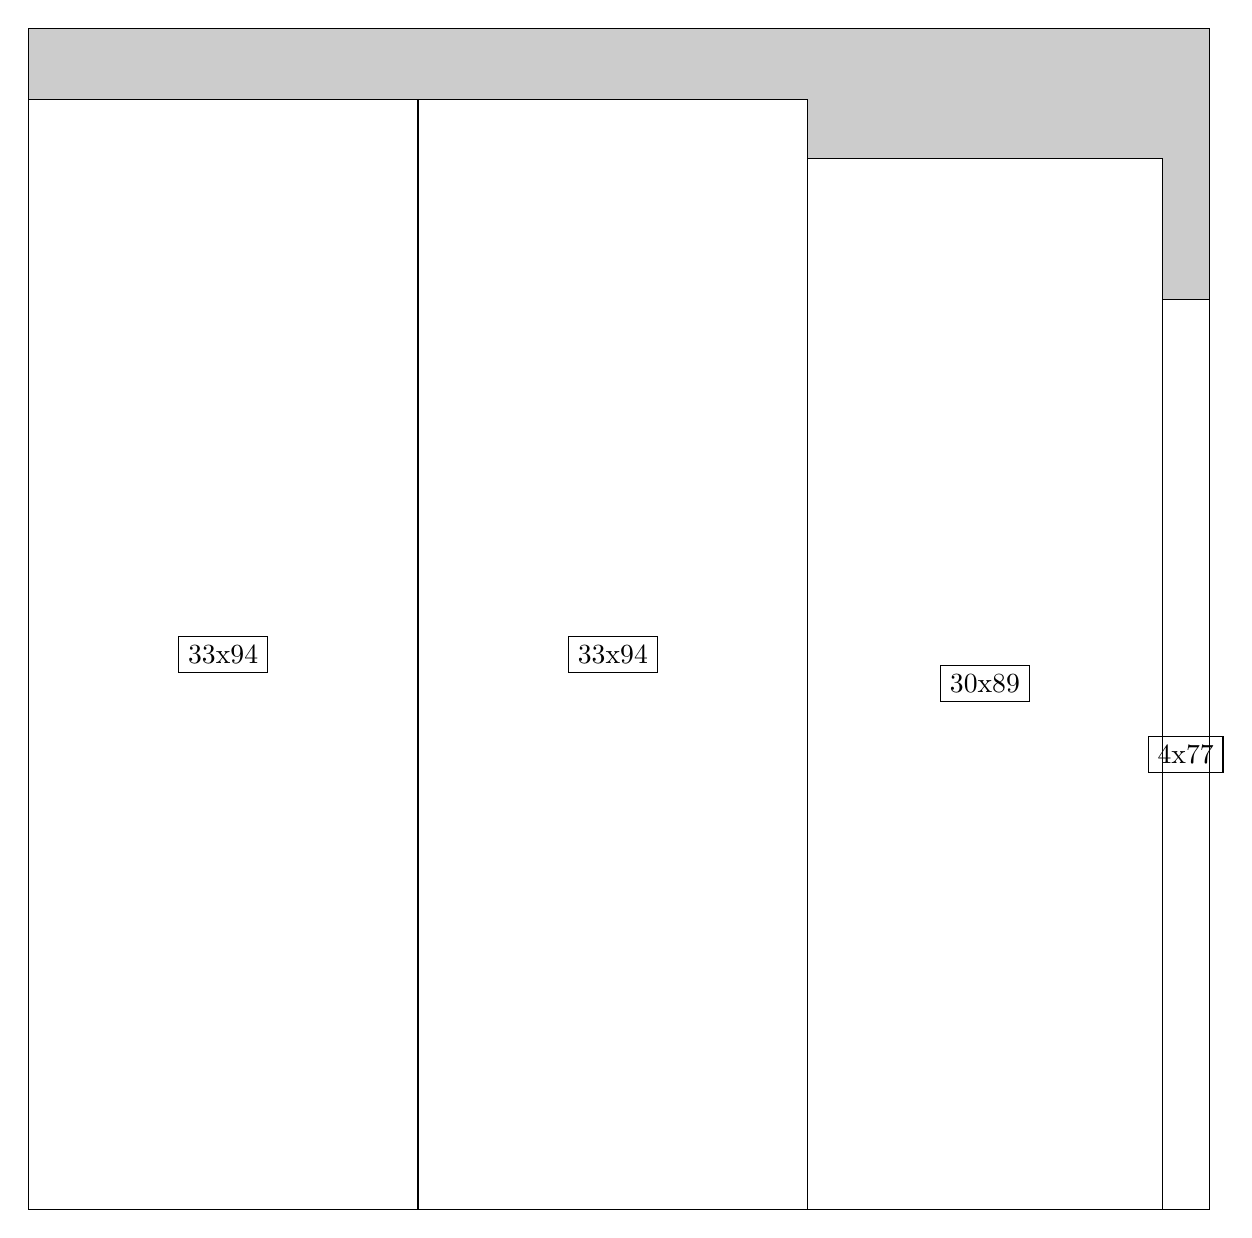
\begin{tikzpicture}[shorten >=1pt,scale=1.0,every node/.style={scale=1.0},->]
\tikzstyle{vertex}=[circle,fill=black!25,minimum size=14pt,inner sep=0pt]
\filldraw[fill=gray!40!white, draw=black] (0,0) rectangle (15.0,15.0);
\foreach \name/\x/\y/\w/\h in {33x94/0.0/0.0/4.95/14.1,33x94/4.95/0.0/4.95/14.1,30x89/9.9/0.0/4.5/13.35,4x77/14.399999999999999/0.0/0.6/11.549999999999999}
\filldraw[fill=white!40!white, draw=black] (\x,\y) rectangle node[draw] (\name) {\name} ++(\w,\h);
\end{tikzpicture}


w =33 , h =94 , x =0 , y =0 , v =3102
\par
w =33 , h =94 , x =33 , y =0 , v =3102
\par
w =30 , h =89 , x =66 , y =0 , v =2670
\par
w =4 , h =77 , x =96 , y =0 , v =308
\par
\newpage


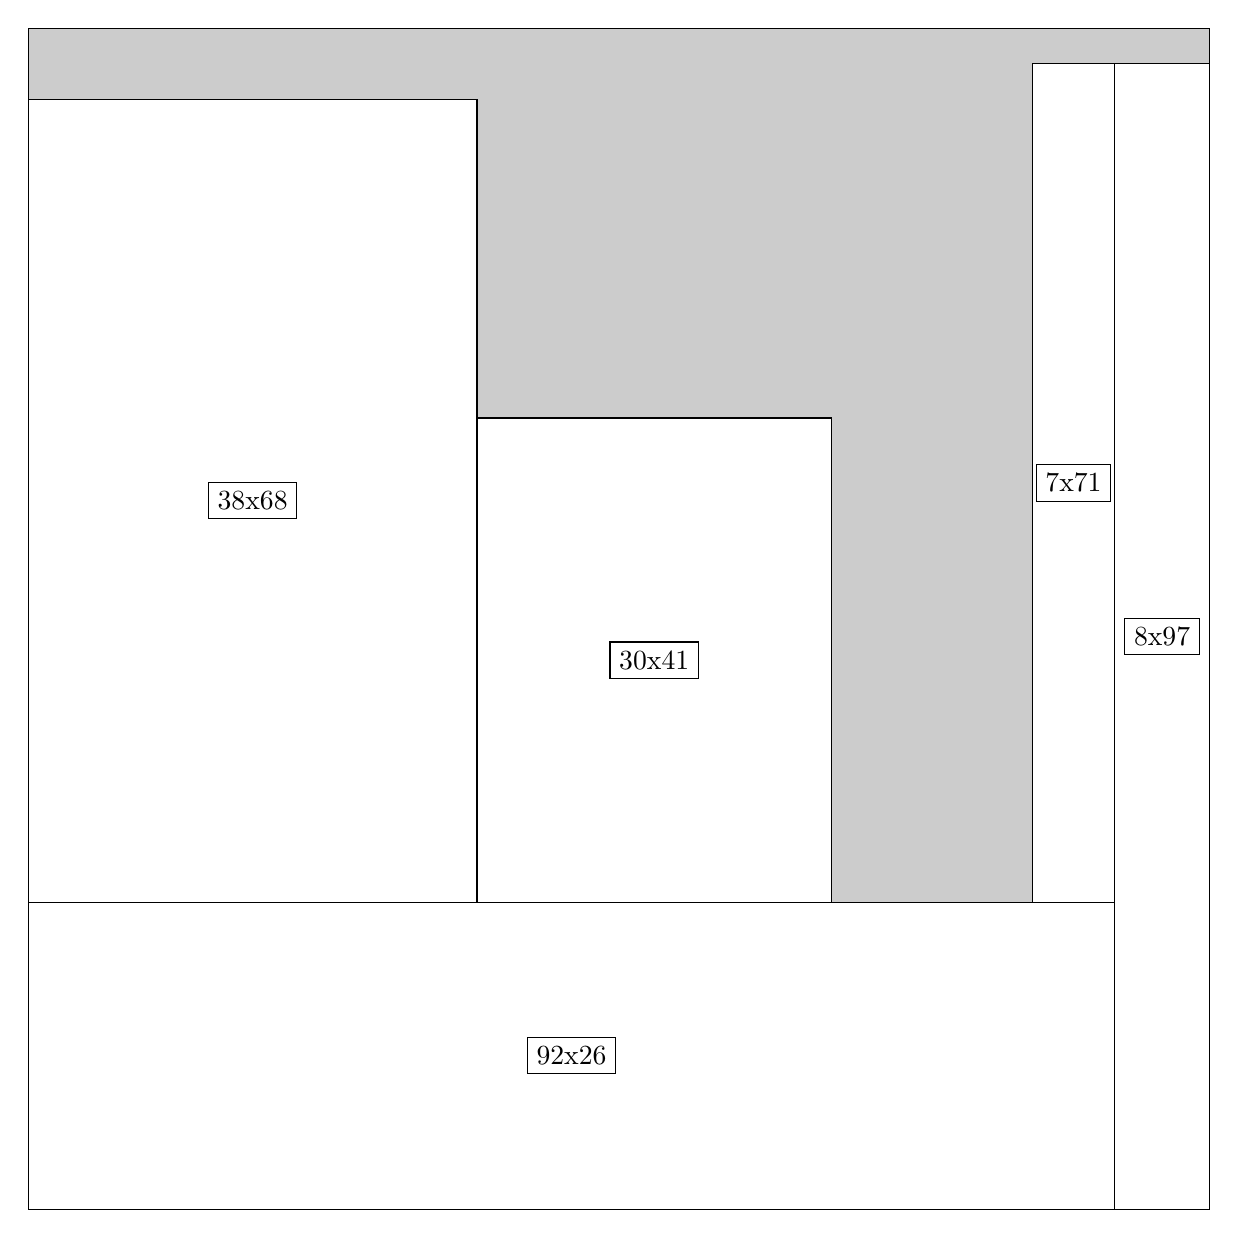
\begin{tikzpicture}[shorten >=1pt,scale=1.0,every node/.style={scale=1.0},->]
\tikzstyle{vertex}=[circle,fill=black!25,minimum size=14pt,inner sep=0pt]
\filldraw[fill=gray!40!white, draw=black] (0,0) rectangle (15.0,15.0);
\foreach \name/\x/\y/\w/\h in {92x26/0.0/0.0/13.799999999999999/3.9,38x68/0.0/3.9/5.7/10.2,30x41/5.7/3.9/4.5/6.1499999999999995,8x97/13.799999999999999/0.0/1.2/14.549999999999999,7x71/12.75/3.9/1.05/10.65}
\filldraw[fill=white!40!white, draw=black] (\x,\y) rectangle node[draw] (\name) {\name} ++(\w,\h);
\end{tikzpicture}


w =92 , h =26 , x =0 , y =0 , v =2392
\par
w =38 , h =68 , x =0 , y =26 , v =2584
\par
w =30 , h =41 , x =38 , y =26 , v =1230
\par
w =8 , h =97 , x =92 , y =0 , v =776
\par
w =7 , h =71 , x =85 , y =26 , v =497
\par
\newpage


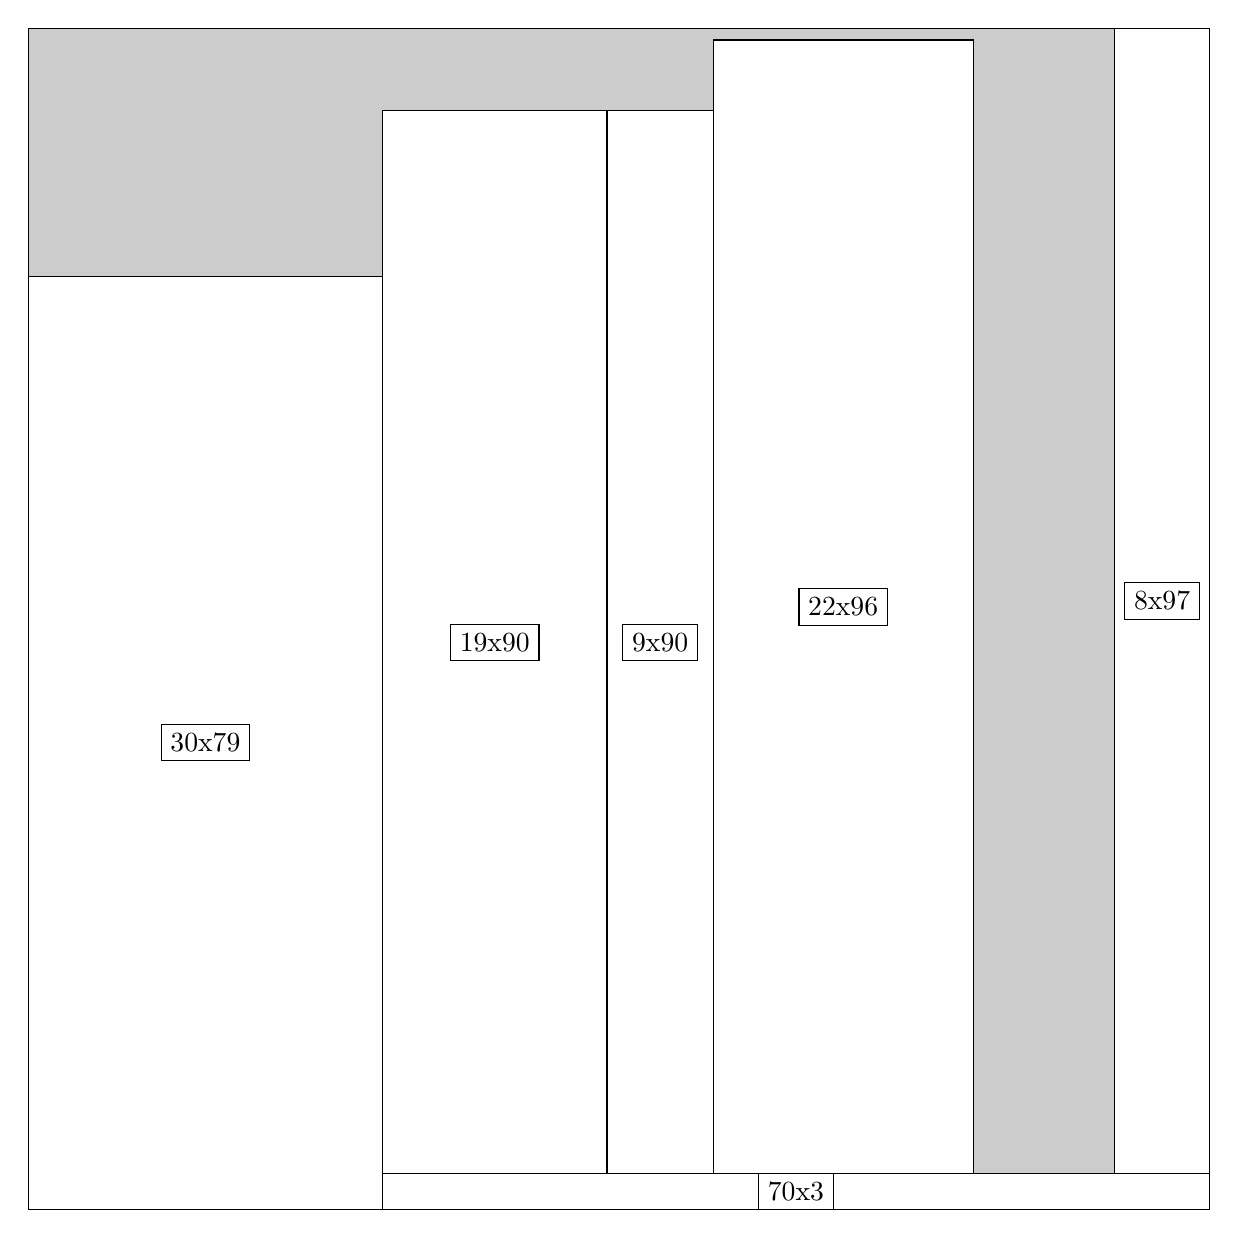
\begin{tikzpicture}[shorten >=1pt,scale=1.0,every node/.style={scale=1.0},->]
\tikzstyle{vertex}=[circle,fill=black!25,minimum size=14pt,inner sep=0pt]
\filldraw[fill=gray!40!white, draw=black] (0,0) rectangle (15.0,15.0);
\foreach \name/\x/\y/\w/\h in {30x79/0.0/0.0/4.5/11.85,22x96/8.7/0.44999999999999996/3.3/14.399999999999999,19x90/4.5/0.44999999999999996/2.85/13.5,9x90/7.35/0.44999999999999996/1.3499999999999999/13.5,8x97/13.799999999999999/0.44999999999999996/1.2/14.549999999999999,70x3/4.5/0.0/10.5/0.44999999999999996}
\filldraw[fill=white!40!white, draw=black] (\x,\y) rectangle node[draw] (\name) {\name} ++(\w,\h);
\end{tikzpicture}


w =30 , h =79 , x =0 , y =0 , v =2370
\par
w =22 , h =96 , x =58 , y =3 , v =2112
\par
w =19 , h =90 , x =30 , y =3 , v =1710
\par
w =9 , h =90 , x =49 , y =3 , v =810
\par
w =8 , h =97 , x =92 , y =3 , v =776
\par
w =70 , h =3 , x =30 , y =0 , v =210
\par
\newpage


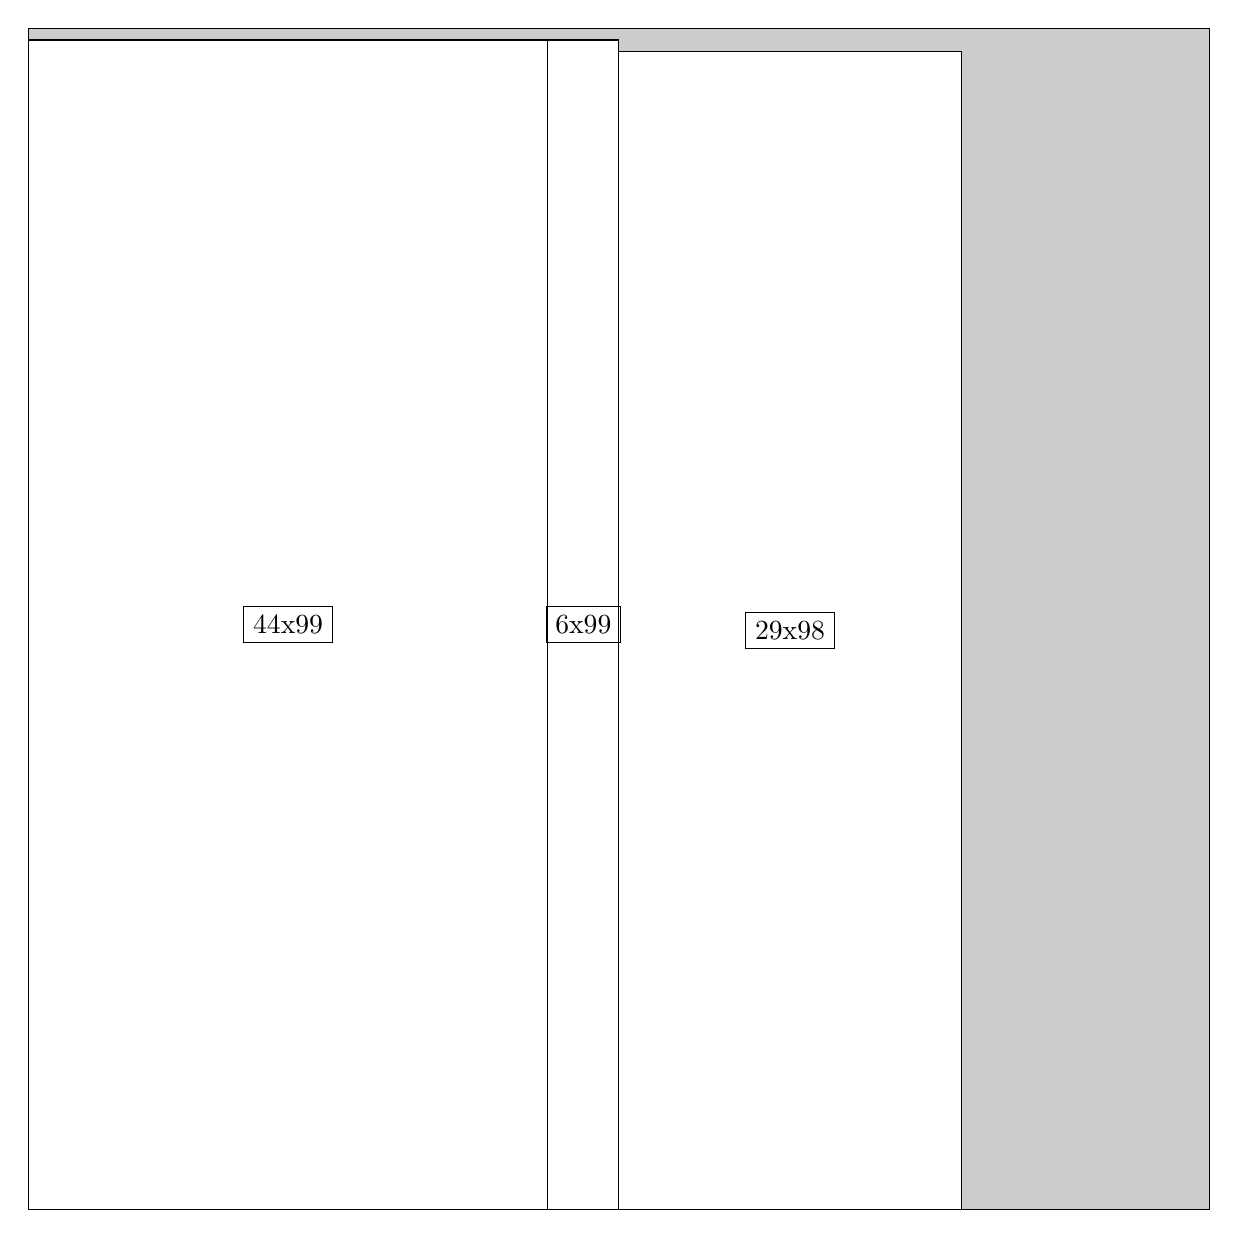
\begin{tikzpicture}[shorten >=1pt,scale=1.0,every node/.style={scale=1.0},->]
\tikzstyle{vertex}=[circle,fill=black!25,minimum size=14pt,inner sep=0pt]
\filldraw[fill=gray!40!white, draw=black] (0,0) rectangle (15.0,15.0);
\foreach \name/\x/\y/\w/\h in {44x99/0.0/0.0/6.6/14.85,29x98/7.5/0.0/4.35/14.7,6x99/6.6/0.0/0.8999999999999999/14.85}
\filldraw[fill=white!40!white, draw=black] (\x,\y) rectangle node[draw] (\name) {\name} ++(\w,\h);
\end{tikzpicture}


w =44 , h =99 , x =0 , y =0 , v =4356
\par
w =29 , h =98 , x =50 , y =0 , v =2842
\par
w =6 , h =99 , x =44 , y =0 , v =594
\par
\newpage


\end{document}